\section{LSTM}
LSTM (abbreviation for Long-short Term Memory) is a variant of recurrent neural network. LSTM seeks to solve vanishing gradient and exploding gradient problem in vanilla recurrent neural network. These problems happen when a training sequence is too long. LSTM introduces gating concept in recurrent neural network. An LSTM contains three gates, an input gate, an output gate, and a forget gate. A forget gate determines when to reset the content of the cell memory. An input and output gate control the flows of input and output of the LSTM respectively.
\begin{figure}[h]
	\centering
	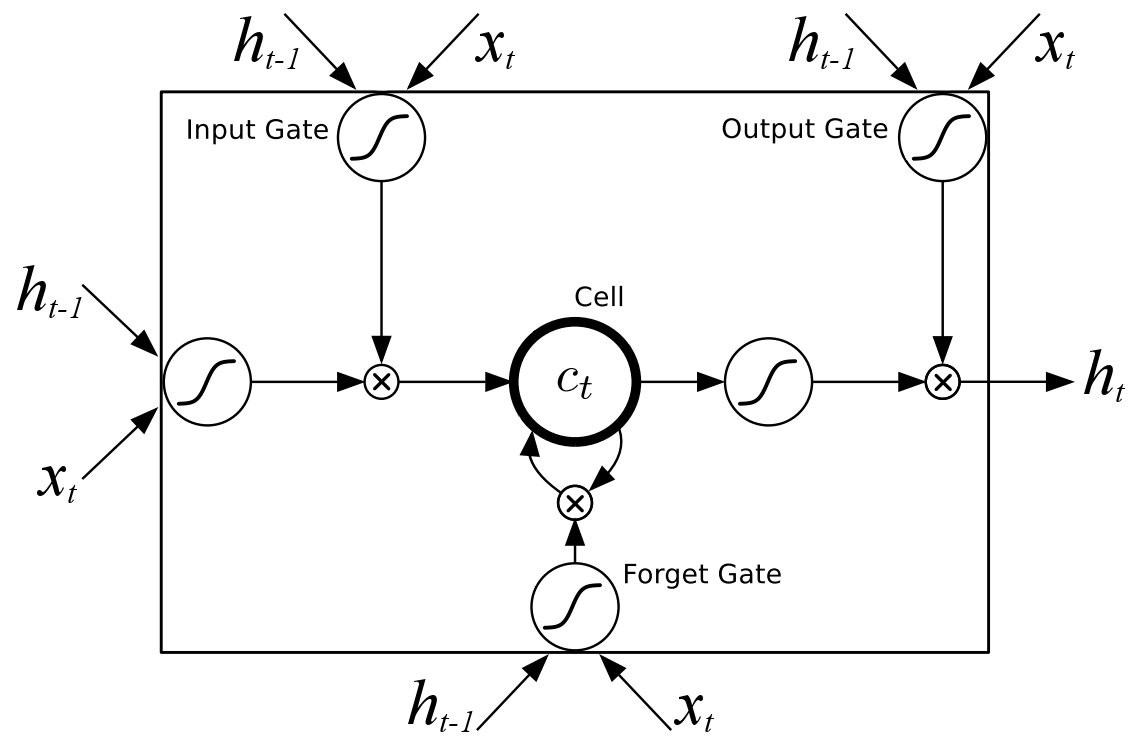
\includegraphics[width=0.85 \textwidth]{assets/lstm.png}
	\caption{An LSTM unit}
	\label{fig:lstm}
\end{figure} \\
We use LSTM unit provided by Caffe\footnote{\href{https://github.com/BVLC/caffe}{Caffe} is developed by Berkeley Vision and Learning Center (BVLC)} framework. It requires CUDA 8 and cuDNN v5.1 from Nvidia, which enable Caffe framework to utilize Nvidia GPU to train a neural network. We used Nvidia GTX 850m to train our LSTM model. This GPU is pretty decent to train a small-sized network. \\ \\
The main idea of this approach is to train each store separately. Training an LSTM model for the entire training set is infeasible as the network model required would be large and our GPU is not powerful enough for it. Since there are 1115 stores, we are going to train 1115 small LSTM models for each store. \\ \\
There are few preprocessing steps that have to be taken before training an LSTM model. First, we need to split the training dataset by store ID since we are training one model for one store. Then, we need to drop \textit{Customers} column as this column is not available in the test dataset. Next, we have to drop \textit{StoreType}, \textit{Assortment}, \textit{HasCompetition}, and \textit{CompetitionDistance} as we are going to train an LSTM model for each store. Finally, normalize the date to $[0,1]$, where $0.0$ indicates 1 Jan 2013, and $1.0$ indicates 17 Sept 2015. \\ \\
The network architecture consists of, in this order, an input layer with 15 features, an LSTM unit, a fully-connected layer, and an output layer. The LSTM unit contains 50 hidden units, and the fully-connected layer contains 50 neurons. The training algorithm used is RMSProp with decaying learning rate. The learning rate update equation is as follows.
\begin{equation}
\label{eq:decay_lr}
\alpha_{t+1} = \frac{\alpha_t}{1 + \gamma t} \text{, where } \gamma \text{ is the decay rate.}
\end{equation}
Base learning rate $\alpha_0$ is $0.001$, learning rate decay $\gamma$ is $10^{-6}$, and RMS decay is $0.9$. The LSTM model is trained for 200 epochs, and the last 50 days of training data of each store are used as validation. At the end of the training, we have 1115 LSTM models. The training duration is approximately four hours. \\ \\
The performance result by this model according to Kaggle, is shown in the table below.
\begin{table}[h]
	\centering
	\caption{LSTM per store result}
	\label{tab:lstm_result}
	\begin{tabular}{|m{100pt}|m{50pt}|}
		\hline
		Private score & 0.15578 \\ \hline
		Public score  & 0.15904 \\ \hline
	\end{tabular}
\end{table}